%%%%%%%%%%%%%%%%%%%%%%%%%%%%%%%%%%%%%%%%%
% Thin Sectioned Essay
% LaTeX Template
% Version 1.0 (3/8/13)
%
% This template has been downloaded from:
% http://www.LaTeXTemplates.com
%
% Original Author:
% Nicolas Diaz (nsdiaz@uc.cl) with extensive modifications by:
% Vel (vel@latextemplates.com)
%
% License:
% CC BY-NC-SA 3.0 (http://creativecommons.org/licenses/by-nc-sa/3.0/)
%
%%%%%%%%%%%%%%%%%%%%%%%%%%%%%%%%%%%%%%%%%

%----------------------------------------------------------------------------------------
%	PACKAGES AND OTHER DOCUMENT CONFIGURATIONS
%----------------------------------------------------------------------------------------

\documentclass[a4paper, 12pt]{article} % Font size (can be 10pt, 11pt or 12pt) and paper size (remove a4paper for US letter paper)

\usepackage[protrusion=true,expansion=true]{microtype} % Better typography
\usepackage{graphicx} % Required for including pictures
\usepackage[utf8]{inputenc}
\usepackage[margin=1.0in]{geometry}
\usepackage{url}
\usepackage{fancyhdr}
\usepackage{amsmath}
\usepackage{setspace}
\usepackage{enumitem}
\setlength\parindent{0pt} % Removes all indentation from paragraphs

\usepackage[T1]{fontenc} % Required for accented characters
\usepackage{times} % Use the Palatino font

\usepackage{listings}
\usepackage{color}
\lstset{mathescape}

\definecolor{dkgreen}{rgb}{0,0.6,0}
\definecolor{gray}{rgb}{0.5,0.5,0.5}
\definecolor{mauve}{rgb}{0.58,0,0.82}

\lstset{frame=tb,
   language=c++,
   aboveskip=3mm,
   belowskip=3mm,
   showstringspaces=false,
   columns=flexible,
   basicstyle={\small\ttfamily},
   numbers=none,
   numberstyle=\tiny\color{gray},
   keywordstyle=\color{blue},
   commentstyle=\color{dkgreen},
   stringstyle=\color{mauve},
   breaklines=true,
   breakatwhitespace=true
   tabsize=3
}
\linespread{1.24} % Change line spacing here, Palatino benefits from a slight increase by default

\makeatletter
\renewcommand{\@listI}{\itemsep=0pt} % Reduce the space between items in the itemize and enumerate environments and the bibliography

\renewcommand\abstractname{Résumé}
\renewcommand\refname{Références}
\renewcommand\contentsname{Table des matières}
\renewcommand{\maketitle}{ % Customize the title - do not edit title and author name here, see the TITLE block below
\begin{center} % Right align

\vspace*{25pt} % Some vertical space between the title and author name
{\LARGE\@title} % Increase the font size of the title

\vspace{125pt} % Some vertical space between the title and author name

{\large\@author} % Author name

\vspace{125pt} % Some vertical space between the author block and abstract
Dans le cadre du cours
\\INF8702 - Infographie avancée
\vspace{125pt} % Some vertical space between the author block and abstract
\\\@date % Date
\vspace{125pt} % Some vertical space between the author block and abstract

\end{center}
}

%----------------------------------------------------------------------------------------
%	TITLE
%----------------------------------------------------------------------------------------

\title{Rapport final: Génération de vague à l'aide de particule} 

\author{\textsc{Guillaume Arruda 1635805\\Raphael Lapierre 1644671} % Author
\vspace{10pt}
\\{\textit{École polytechnique de Montréal}}} % Institution

\date{8 Décembre 2015} % Date

%----------------------------------------------------------------------------------------

\begin{document}

\thispagestyle{empty}
\clearpage\maketitle % Print the title section
\pagebreak[4]
\tableofcontents
\pagebreak[4]
%------------------------------------------------------------------------------------- ---
%	En tête et pieds de page 
%----------------------------------------------------------------------------------------

\setlength{\headheight}{15.0pt}
\pagestyle{fancy}
\fancyhead[L]{INF8702}
\fancyhead[C]{}
\fancyhead[R]{Rapport final}
\fancyfoot[C]{\textbf{page \thepage}}

%----------------------------------------------------------------------------------------
%	ESSAY BODY
%----------------------------------------------------------------------------------------
\section*{Problématique}
\section*{Théorie}
\section*{Implémentation}
\subsection{Introduction au moteur graphique}
Le moteur graphique a été écrit pour nous familiariser avec OpenGL 4.4. 
\subsection*{Génération et gestion des particules}
\subsection*{Création de la carte de hauteurs}
\subsection*{Réflection}
\subsection*{Réfraction}
\section*{Conclusion}
\section*{Références}
\begin{figure}
	\centering
	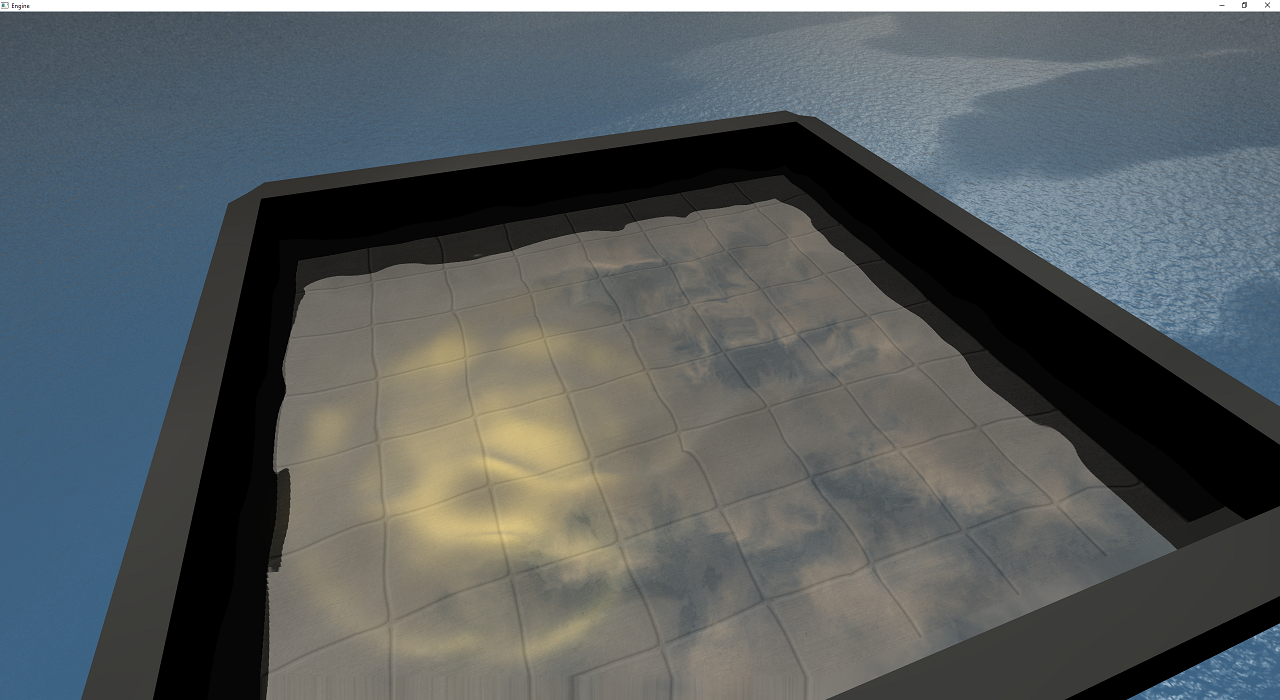
\includegraphics[width=0.9\textwidth]{./PhotoRapport/EffetFinal.png}
	\caption{Effet final}
	\label{EffetFinal}
\end{figure}
\begin{figure}
	\centering
	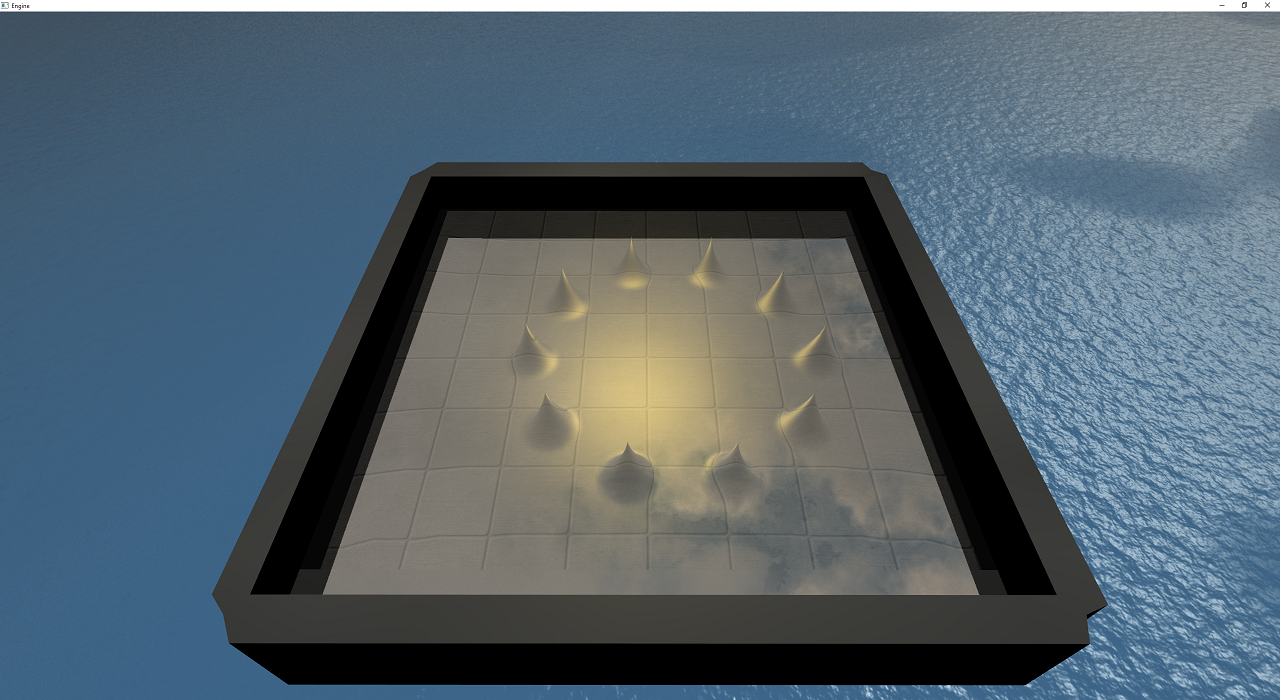
\includegraphics[width=0.9\textwidth]{./PhotoRapport/NoSubdivide.png}
	\caption{Sans subdivision}
	\label{NoSubdivide}
\end{figure}
\begin{figure}
	\centering
	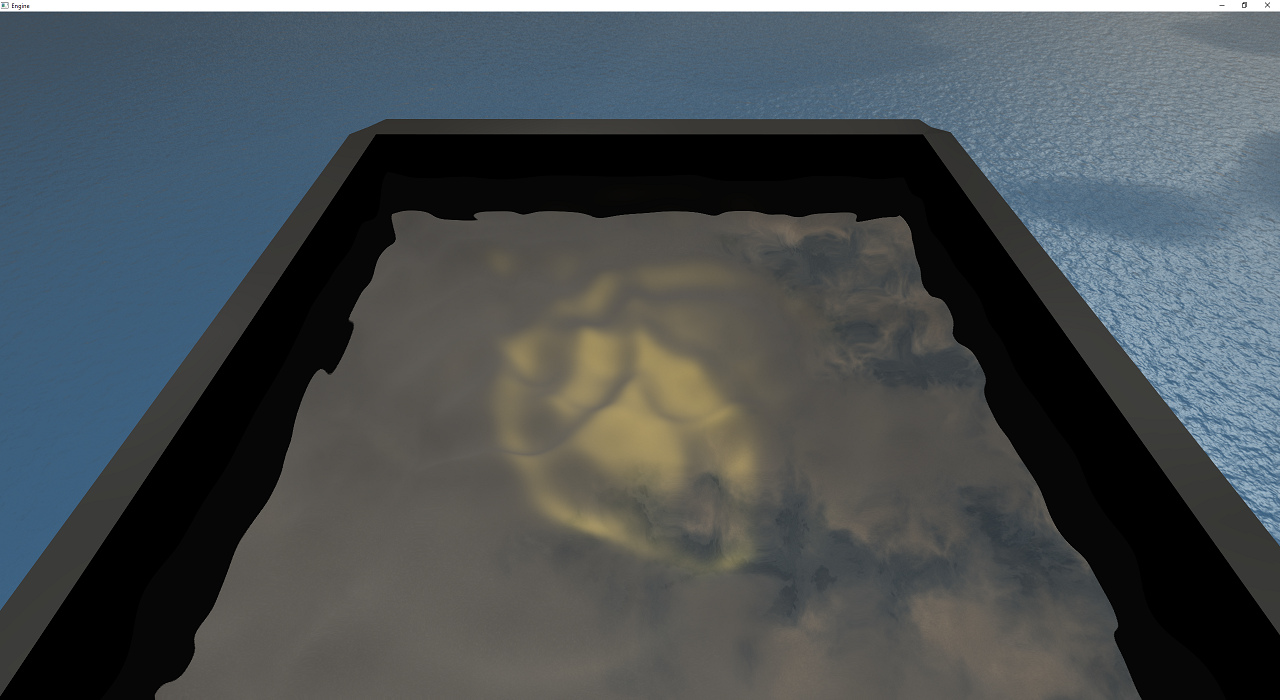
\includegraphics[width=0.9\textwidth]{./PhotoRapport/Reflection.png}
	\caption{Reflection}
	\label{Reflection}
\end{figure}
\begin{figure}
	\centering
	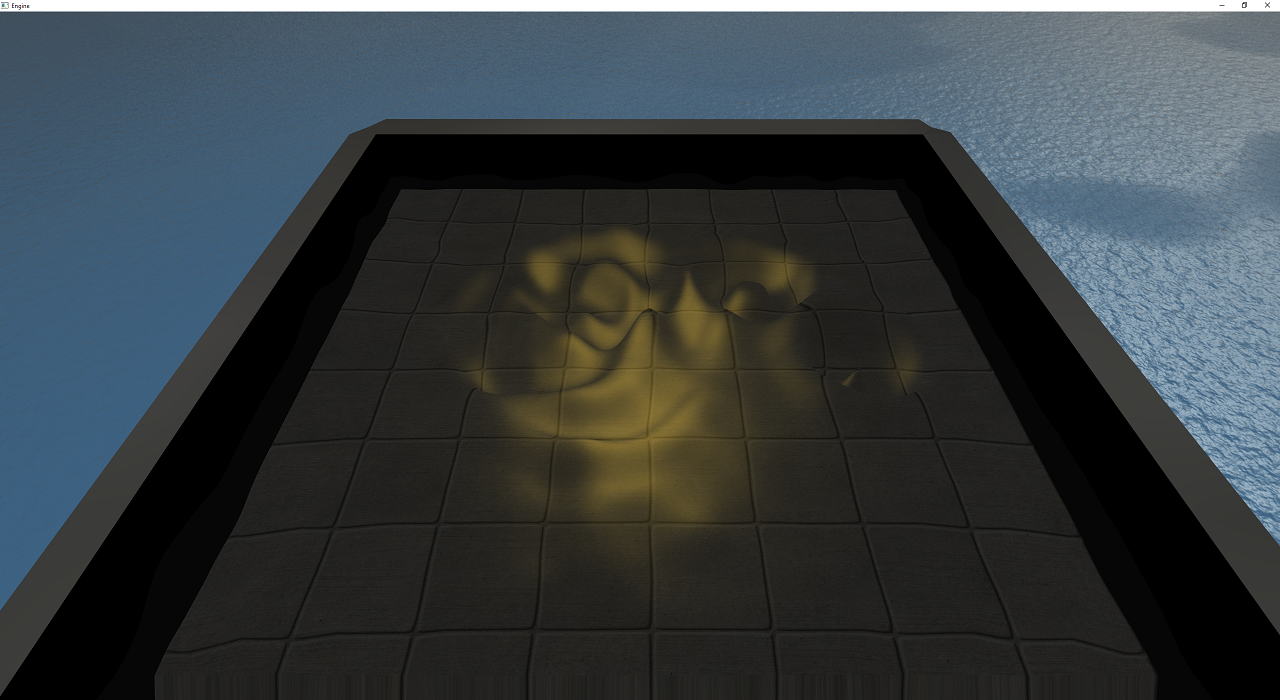
\includegraphics[width=0.9\textwidth]{./PhotoRapport/Refraction.png}
	\caption{Refraction}
	\label{Refractopm}
\end{figure}
\begin{figure}
	\centering
	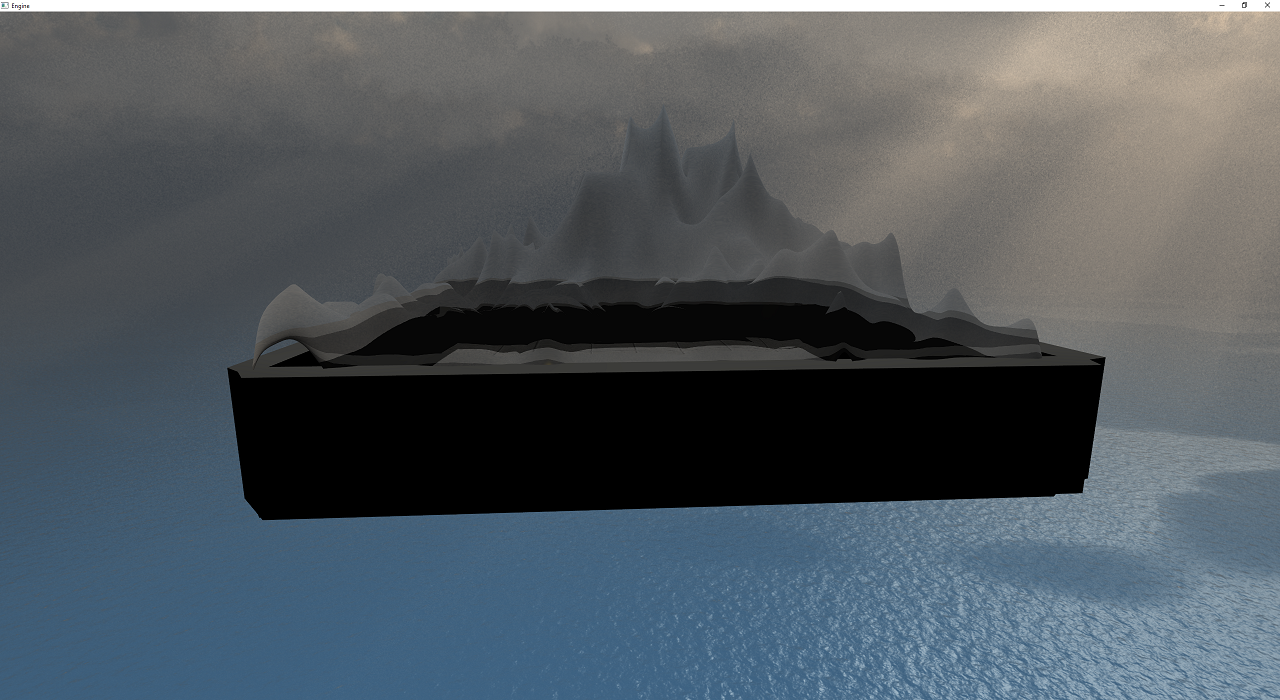
\includegraphics[width=0.9\textwidth]{./PhotoRapport/WaterConservation.png}
	\caption{Conservation d'eau}
	\label{WaterConservation}
\end{figure}
%----------------------------------------------------------------------------------------
\end{document}
